\chapter{Résultats} \label{chap:resultats}

Introduction et annonce du plan du chapitre.
\lipsum[1] % génère un paragraphe (à supprimer)

\section{Section 1} \label{sec:titre_section1}

Paragraphe.
\lipsum[1] % génère un paragraphe (à supprimer)


\section{Section 2} \label{sec:titre_section2}

Paragraphe.
\lipsum[1-2] % génère deux paragraphes (à supprimer)

Les statistiques... (tableau~\ref{tab:cellules_fusionnees}).

\begin{table}[H]
    \singlespacing
    \begin{threeparttable}
    \caption{Tableau avec des cellules fusionnées}
    \label{tab:cellules_fusionnees}
    \renewcommand{\arraystretch}{1.2}
    \begin{tabular}{lll}
        \hline
        \textbf{Type de variable} & \textbf{Nom} & \textbf{Abréviation} \\
        \hline
        Dépendante & Dioxyde d'azote ($\mu$g/m$^3$) & NO$_2$ \\
        \hline
        Variable de contrôle & Température ($^\circ$C) & Temp \\
                             & Humidité (\%) & Humid \\
                             & Vitesse du vent (km/h) & Vitesse \\
        \hline
        Variable explicative & Nombre d'intersections (N) & Inters \\
                             & Localisation géographique & XY \\
                             & Vitesse (km/h) & Vitesse \\
        \hline
    \end{tabular}
    \end{threeparttable}
\end{table}

Nam dui ligula, fringilla a, euismod sodales, sollicitudin vel, wisi. Morbi auctor lorem non justo.
Nam lacus libero, pretium at, lobortis vitae, ultricies et, tellus. Donec aliquet, tortor sed accumsan bibendum, erat ligula aliquet magna, vitae ornare odio metus a mi. Morbi ac orci et nisl hendrerit mollis. Suspendisse ut massa. Cras nec ante. Pellentesque a nulla. Cum sociis natoque penatibus et magnis dis parturient montes, nascetur ridiculus mus (figure~\ref{fig:plusieurs_vignettes}).

\begin{figure}[H]
    \centering
    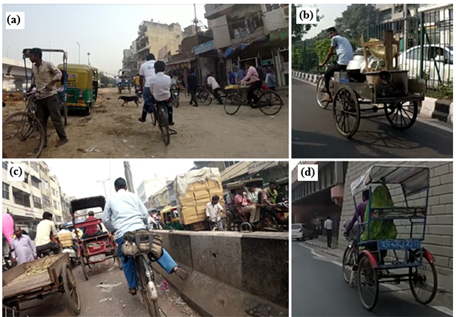
\includegraphics[width=0.8\textwidth]{figures/figureavecplusieursvignettes.png}
    \caption[Figure avec plusieurs vignettes]{Figure avec plusieurs vignettes. \textbf{(a)} Description. \textbf{(b)} Description. \textbf{(c)} Description. (d) Description. Figure adaptée de \textcite[2]{apparicio2021cycling}.}
    \label{fig:plusieurs_vignettes}
\end{figure}

